%%%%%%%%%%%%%%%%%%%%%%%%%%%%%%%%%%%%%%%%%%%%%%%%%%%%%%%%%%%%%%%%%%%%%%%%%%%%
% AGUtmpl.tex: this template file is for articles formatted with LaTeX2e,
% Modified March 2013
%
% This template includes commands and instructions
% given in the order necessary to produce a final output that will
% satisfy AGU requirements.
%
% PLEASE DO NOT USE YOUR OWN MACROS
% DO NOT USE \newcommand, \renewcommand, or \def.
%
% FOR FIGURES, DO NOT USE \psfrag or \subfigure.
%
%%%%%%%%%%%%%%%%%%%%%%%%%%%%%%%%%%%%%%%%%%%%%%%%%%%%%%%%%%%%%%%%%%%%%%%%%%%%
%
% All questions should be e-mailed to latex@agu.org.
%
%%%%%%%%%%%%%%%%%%%%%%%%%%%%%%%%%%%%%%%%%%%%%%%%%%%%%%%%%%%%%%%%%%%%%%%%%%%%
%
% Step 1: Set the \documentclass
%
% There are two options for article format: two column (default)
% and draft.
%
% PLEASE USE THE DRAFT OPTION TO SUBMIT YOUR PAPERS.
% The draft option produces double spaced output.
%
% Choose the journal abbreviation for the journal you are
% submitting to:

% jgrga JOURNAL OF GEOPHYSICAL RESEARCH
% gbc   GLOBAL BIOCHEMICAL CYCLES
% grl   GEOPHYSICAL RESEARCH LETTERS
% pal   PALEOCEANOGRAPHY
% ras   RADIO SCIENCE
% rog   REVIEWS OF GEOPHYSICS
% tec   TECTONICS
% wrr   WATER RESOURCES RESEARCH
% gc    GEOCHEMISTRY, GEOPHYSICS, GEOSYSTEMS
% sw    SPACE WEATHER
% ms    JAMES
% ef    EARTH'S FUTURE
%
%
%
% (If you are submitting to a journal other than jgrga,
% substitute the initials of the journal for "jgrga" below.)

\documentclass[draft,grl]{AGUTeX}
% To create numbered lines:

% If you don't already have lineno.sty, you can download it from
% http://www.ctan.org/tex-archive/macros/latex/contrib/ednotes/
% (or search the internet for lineno.sty ctan), available at TeX Archive Network (CTAN).
% Take care that you always use the latest version.

% To activate the commands, uncomment \usepackage{lineno}
% and \linenumbers*[1]command, below:

\usepackage{lineno}
\usepackage{amssymb}
\usepackage{amsmath}
\usepackage{textcomp}
\usepackage[super]{nth}
\linenumbers*[1]

%  To add line numbers to lines with equations:
%  \begin{linenomath*}
%  \begin{equation}
%  \end{equation}
%  \end{linenomath*}
%%%%%%%%%%%%%%%%%%%%%%%%%%%%%%%%%%%%%%%%%%%%%%%%%%%%%%%%%%%%%%%%%%%%%%%%%
% Figures and Tables
%
%
% DO NOT USE \psfrag or \subfigure commands.
%
%  Figures and tables should be placed AT THE END OF THE ARTICLE,
%  after the references.
%
%  Uncomment the following command to include .eps files
%  (comment out this line for draft format):
\usepackage[final]{graphicx}
%
%  Uncomment the following command to allow illustrations to print
%   when using Draft:
%  \setkeys{Gin}{draft=false}
%
% Substitute one of the following for [dvips] above
% if you are using a different driver program and want to
% proof your illustrations on your machine:
%
% [xdvi], [dvipdf], [dvipsone], [dviwindo], [emtex], [dviwin],
% [pctexps],  [pctexwin],  [pctexhp],  [pctex32], [truetex], [tcidvi],
% [oztex], [textures]
%
% See how to enter figures and tables at the end of the article, after
% references.
%
%% ------------------------------------------------------------------------ %%
%
%  ENTER PREAMBLE
%
%% ------------------------------------------------------------------------ %%

% Author names in capital letters:
\authorrunninghead{DAY ET AL.}

% Shorter version of title entered in capital letters:
\titlerunninghead{COUPLED MEIYU AND JET VARIABILITY}

%Corresponding author mailing address and e-mail address:
\authoraddr{Corresponding author: Jesse Day, University of California Berkeley, Department of Earth and Planetary Science, College of Letters and Science; 307 McCone Hall, Berkeley, CA 94720, USA. (jessed@berkeley.edu)}

\begin{document}

%% ------------------------------------------------------------------------ %%
%
%  TITLE
%
%% ------------------------------------------------------------------------ %%


\title{Covariance of Meiyu Front and Tropospheric Jet Variability on Daily and Interannual time scales}

%% ------------------------------------------------------------------------ %%
%
%  AUTHORS AND AFFILIATIONS
%
%% ------------------------------------------------------------------------ %%


%Use \author{\altaffilmark{}} and \altaffiltext{}

% \altaffilmark will produce footnote;
% matching \altaffiltext will appear at bottom of page.

\authors{Jesse A. Day,\altaffilmark{1}
Jacob Edman,\altaffilmark{1} Inez Fung \altaffilmark{1}, and
Weihan Liu\altaffilmark{1}}

\altaffiltext{1}{Department of Earth and Planetary Science, University of California Berkeley, Berkeley, California, USA.}

%% ------------------------------------------------------------------------ %%
%
%  ABSTRACT
%
%% ------------------------------------------------------------------------ %%

% >> Do NOT include any \begin...\end commands within
% >> the body of the abstract.

\begin{abstract}
This abstract must be 150 words or less. The contents of the abstract count towards the total word count.
\end{abstract}

%  and tables.

\begin{article}

%% ------------------------------------------------------------------------ %%

%% ------------------------------------------------------------------------ %%

\section{Introduction}
 
 China receives about 60\% of its rainfall from May to August, known collectively as the East Asian summer monsoon. The period of peak rainfall within this monsoon features a northward-migrating front known as the Meiyu front (lit. ``Plum rains''  -- capitalize front?), and lasts roughly from early June to mid-July (``Meiyu Season''). A growing volume of evidence suggests a shift in mean rainfall patterns over China beginning in the late 1970s, with increased flooding in the south and droughts in the north (the ``South Flood North Drought''). A permanent change would have major humanitarian impacts on the densely-populated eastern Chinese plain, where a sizable fraction of the population depends on agriculture. The Chinese government has already embarked on a costly engineering project to reroute water from the Yangtze to the Yellow River, the South-North Water Transfer Project.
 
	The complex atmospheric dynamics of the East Asian summer monsoon remain a source of debate \citep{Sampe2010,Chen2014}. The behavior of the Meiyu front has been discussed in the seasonal mean\citep{Ding2005}, and in relation to interannual rainfall variability \citep{Kosaka}. However, to our knowledge, no comprehensive statistics of daily Meiyu behavior exist. We have developed an algorithm to compile a 57-year climatology (1951-2007) of frontal events in China (hereafter referred to as Meiyu events) based on the APHRODITE rain gauge product. In addition, we test the covariance of daily Meiyu behavior with that of the tropospheric jet, using an existing database from \citet{Schiemann2009}. Past work has compared jet and Meiyu variability over shorter time periods or with coarse resolution\cite{Liang1998}, but none has systematically compared the two.  Finally, given our daily Meiyu climatology, we determine whether there are apparent changes in behavior over the 57 years, and whether these also correspond to changes in jet behavior.

%consider adding a sentence in the previous paragraph that explains why the jet should be related to Meiyu behavior - existing simple reference?
%Current theory suggests that the tropospheric jet plays a major role in Meiyu formation, either by zonal advection of sensible heat from the Tibetan Plateau upwind \citep{Sampe2010}, or as part of the orographically forced circulation that produces meridional wind convergence over China\citep{Chen2014}.

% Paper may be short enough that it is unnecessary to delineate what each section contains.
%	In the following text we seek to achieve the following objectives: 1) Define an objective climatology of the Meiyu front; 2) Show the positions of the tropospheric jet associated with different configurations of the tropospheric jet; 3) Show that the Meiyu front and tropospheric jet covary on a daily scale; and 4) Suggest a dynamic lens to understand the observed climatology of Meiyu front and jet.
	
\section{Data sets}
	The analysis contained in this paper relies on two data sets, APHRODITE and Schiemann et al's database of jet counts. APHRODITE (Asian Precipitation - Highly-Resolved Observational Data Integration Towards Evaluation of the Water Resources) \citep{Yatagai2012}. The APHRO\_MA\_V1101 product includes 57 years (1951-2007) of daily precipitation (PRECIP product, units mm day$^{-1}$) and station coverage (RSTN product) on a .25\textdegree\ $\times$ .25\textdegree\ grid (roughly 25 km spacing) between 60\textdegree E-150\textdegree E and 15\textdegree S-55\textdegree N. We focus on the subregion from 100E-123E and 20N-40N as the area of occurrence of Meiyu events. Rain gauge products present an analytical challenge because the distribution of stations is uneven in space and changes with time. Station density over eastern China improves beginning in the 1970s from X to Y (INSERT ACTUAL NUMBERS). However, the spacing of stations generally does not exceed 100 km, which should be more than sufficient to resolve the macroscopic scale of a frontal event.

	For tropospheric jet variability, we employ a database based on ERA-40 reanalysis data developed by \citet{Schiemann2009}. Their database includes every appearance of a tropospheric jet in East Asia for 1958-2001 at 6-hourly intervals using simple criteria: Positive zonal wind and local maximum in excess of 30 m/s. We have modified Schiemann et al.'s algorithm in several respects: ...

.
	
\section{Meiyu Climatology}
\subsection{Algorithm}

%I am debating the best way of showing the algorithm - other options: Simply write it out in one dreary paragraph, or use a diagram. If diagram, have to be careful since each figure counts as 500 words.

\textbf{List version}

For each day from 1 January 1951 to 31 December 2007 (20,819 total), the algorithm determines whether a frontal event is present or not inside the window of 105-123E and 20-40N, and if it exists returns its properties. In addition, it is observed that some days feature two frontal events. If a primary event is detected, the algorithm therefore checks for a secondary fit as well. The algorithm follows the subsequent checklist:

\begin{enumerate}
	\item The maximum daily rainfall for each longitude is found. If there exists a 5\textdegree continuous chain of maxima (20 points in a row) exceeding 10 mm/day, we proceed to step 2 and attempt a fit. Otherwise, the day is thrown out.
	
	\item A weighted least-squares linear fit of the \textit{latitudes} of the maxima is attempted, using the intensity of the maxima as weight.
	
	\item A recursive algorithm converges on a best estimate. In each iteration, we find a new set of maxima within \textit{k} degrees of the previous best fit line, and again repeat the weighted linear fit in step 2. $k$ is progressively decreased with each iteration.
	
	\item Using our final best estimate from step 3, we define the ``quality score'' $Q$ as the fraction of total daily precipitation that falls within 5 degrees of this fit line.
	
	\item As mentioned, we check for a secondary front. We remove all precipitation within the primary front and again apply the front criterion in step 1 to the leftover rainfall map. If passed, steps 2-4 are repeated to find a best estimate for a secondary front.
	
	\item If a secondary front is found, two additional quality scores $Q_1$ and $Q_2$ are determined. $Q_1$ is defined as the fraction of rainfall contained in the primary front \textit{after removing all rainfall associated with the secondary front}. Likewise $Q_2$ is the Q score of the second front after removing all rainfall from the primary front.
			
\end{enumerate} 
	
In some cases, a fit will be achieved, but its quality will be too poor to include in our statistics. To check for this scenario, we use the quality scores $Q$, $Q_1$ and $Q_2$, and the ``Taiwan fraction'' (TW), defined as the percentage of daily rainfall that falls on the island of Taiwan. If $TW > 20\%$, the day is thrown out. Such days are dominated by a local storm reaching Taiwan and rarely exhibit a strong front. Subsequently there are two ways a day may be included: 
	
\begin{enumerate}
	\item if $Q>.6$, the day is included in our statistics. If $Q_2$ also is greater than .6, the day will be classified as a double front day.
		
	\item If $Q<.6$, a day can only be included if both $Q_1 \mathrm{\textbf{ and }} Q_2 > .6$. In such cases, the quality of fit is initially obscured by the presence of multiple fronts. We classify the day as a double front day.
\end{enumerate}	
		
	In practice, days with secondary fronts constitute a small fraction of all days ($>$ 5\%) but are more common during certain seasons.
		
%Previous attempt at a paragraph explanation - is it acceptable to do a numbered list in a scientific paper?
%	We develop an adaptive algorithm to detect the position of the Meiyu front on a given day. For each day from 1951 to 2007 (20819 days total), we first find the quantity and latitude of maximum rainfall for each longitude point. Then, we use the simple criterion of there being a 5 degree continuous chain of maxima over 10 mm/day (20 consecutive cells). We then try to linearly fit these maxima, excluding any maximum that is more than 5 degrees of latitude away from the precipitation centroid given by $<L> =\frac{\sum P_i y_i}{\sum P}$. Next using, this first fit as starting point, we now find the maxima within a $n$-degree latitude window of the best fit line, where we progressively shrink $n$ with each iteration. The choice of $n$ does not greatly impact fit quality. In our experiment, we repeated the fit for $n$= ... . Given a final fit, we report the latitude of the front at 105\textdegree E, the mean intensity of rainfall along the center of its axis and the tilt (in degrees). We also report a quality score $Q$ which indicates the percentage of rainfall that falls within 3 degrees of our best fit line, such that statistical calculations can be repeated only days with a clear front for the purpose of confirmation. 

%new version of paragraph
	\textbf{Paragraph version}

	For each day from January 1 1951 to December 31 2007 (20,819 days at all) we determine whether there is a frontal event, whether there is an additional secondary front, and the characteristics of each. To detect a front, we find the maximum daily rainfall at each longitude inside the window 105-123\textdegree E and 20-40\textdegree N. If a 5\textdegree continuous chain of maxima exceeds 10 mm/day, we seek a fit; otherwise the day is discarded. The fitting algorithm performs a linear least-squares fit of the \textit{latitudes} of each of the maxima, weighted by the intensity of the maximum. Next, we use a recursive fit wherein we find a new set of maxima, requiring that they be within $n$ degrees of the previous best fit line. $n$ is progressively decreased to tighten the window and converge on an optimal fit. Given this fit, we can calculate a quality score $Q$, which is the percentage of total rainfall in our window that falls within 5 degrees of our best fit line. A score of $Q > .6$ constitutes a good score, as further explained below.
	
	In addition, we determine from observation that some days feature two separate bands of strong rainfall. We would like to include such events. Therefore, after fitting a primary event, we check for a secondary event by removing the rainfall associated with the first best fit line, and then repeating all of the steps of the previous paragraph. If a secondary event is detected, we may define two extra quality scores $Q_1$ and $Q_2$, where $Q_1$ is the percentage of rainfall within \textit{after removing rainfall associated with the secondary fit}, and $Q_2$ likewise is the Q score of the secondary fit after removing rainfall from the primary fit.
	
	Finally, in some cases our front criterion will be satisfied, but we are not able to achieve a good fit. We use the quality scores $Q$, $Q_1$ and $Q_2$ to check for this case, as well as one additional metric, the ``Taiwan fraction'' ($TW$), defined as the percentage of daily rainfall that falls on Taiwan. First of all, all days where $TW > 20\%$ are thrown out. Such days are dominated by a local storm reaching Taiwan, and rarely exhibit a coherent front. Subsequently there are two ways a day may be included: 
	
	\begin{enumerate}
		\item if $Q>.6$, the day is included in our statistics. If $Q_2$ also is greater than .6, the day will be classified as a double front day.
		
		\item If $Q<.6$, a day can only be included if both $Q_1 \mathrm{\textbf{ and }} Q_2 > .6$. In such cases, the quality of fit is initially obscured by the presence of multiple fronts. We classify the day as a double front day.
	\end{enumerate}	
		
	In practice, days with secondary fronts constitute a small fraction of all days ($>$ 5\%) but are more common during certain seasons.
	
\subsection{Statistics}	

	Figure 1a reproduces a plot similar to Ding and Chan's 200x paper, but focusing more narrowly on eastern China.  Figure 1b shows a H\"ovmoller diagram of the latitudes occupied by the Meiyu Front over all 57 years, including both primary and secondary events, with a 5-day and 2\textdegree smoothing. It can be seen that mean rainfall and Meiyu occurrence are not entirely equivalent. For instance, the August peak in southern China rainfall (about 20\textdegree N) does not correspond to a surge in Meiyu events. Certain periods of particular behavior can be discerned: . These correspond to Ding and Chan's ... Table 1 shows the mean characteristics of fronts in each of these periods and their variance.
	
	%the following were my observations from the previous version of Figure 1 - may no longer be accurate, but saving them just in case.
	%Four local maxima of Meiyu events can be observed: 1) A "pre-Meiyu" from May 1-31 over southern China (Ding and Chan's first position); 2) Meiyu Season, in which the preferred latitude of the front shifts by almost ten degrees from June 1-July 15 (Ding and Chan stage 2); 3) A "post-Meiyu" of persistent  4) Cyclone season over Southern China. The storms during season 4 can be distinguished from earlier Meiyu events in southern China because their propagation direction is westward, opposite to eastward Meiyu storms. The combination of stages 3 and 4 corresponds to the third stage of the Meiyu in Ding and Chan, but only the core of Meiyu season (their stage 2) features significant front migration. Figure 2 shows that even in winter, rainfall events in China tend to be frontal, but their frequency increases up to almost 100\% during Meiyu Season, and a surge in intensity can be seen around June 1 where mean rainfall along the front exceeds 25 mm/day. The mean tilt of the front is approximately 8 degrees.
	
	We test for the existence of statistically significant differences between 1951-1979 and 1980-2007 for each of the time periods mentioned above.
	
\section{Preferred jet positions}
	
%snippet
%A new paleoclimate study proposes the tropospheric jet as an indicator of past rainfall patterns in China \citep{Nagashima2011}\citep{Nagashima2013}. The authors study a marine sediment core in the Sea of Japan, downstream from both the Taklamakan Desert and Gobi Desert, and are able to differentiate between dust from each of these sources using electron spin resonance (ESR) and grain size. In the present day, Gobi Desert dust is only advected during spring before the tropospheric jet passes north of the Tibetan Plateau and \citep{Roe2009}, whereas the mechanism of transport of Taklamakan Desert dust remains active in summer when the jet occupies a low variability position on the northern flank of the Tibetan Plateau. Therefore, they attribute increases in Gobi Desert dust to longer springs and shorter summers. Since Holocene changes in precipitation match the timing of abrupt changes in their record, they therefore conclude that the tropospheric jet controls precipitation variability over millennial time scales.
-> The westerly jet and rainfall are argued to covary on paleoclimate timescales \citep{Nagashima2011}\citep{Nagashima2013}.
	
	Monthly changes in the position of the jet have previously been reported in \citet{Schiemann2009}, and we do not repeat them here. It is worth noting that the pre-Meiyu in May corresponds to a time of great jet variability, whereas June features a discernible but meandering jet, and the post-Meiyu corresponds to very low variability in jet position during July and August.
	
		Finally, we use our knowledge of daily Meiyu positions to isolate preferred configurations for different dates, as well as probability distributions of the tropospheric jet associated with each configuration. If a robust change in mean jet progression is detected, we may be able to isolate a corresponding shift in Meiyu distribution that may have previously gone unnoticed due to extreme temporal variability in the data.
		
			We first attempt to define a transition date from spring to summer behavior in the jet database, and equivalently from Meiyu Season to post-Meiyu in our new catalog. Preliminary evidence suggests a long-term perturbation in mean jet path in East Asia from the 1960s to present with later onset of summer jet and shorter total duration of summer jet. In our Meiyu database it is more difficult to extract an exact transition date due to high-frequency variability in space and time. However, we observe an apparent shift in the timing of northward progression of the Meiyu Front between 1951-1970 and 1988-2007. If both databases demonstrate a robust decadal shift, they may provide an explanation for the anecdotal South Wet-North Dry pattern of rainfall change.


	
% which more interesting - chronological jet or position related? try both?

%chronological
%jet corresponding to chronology
%pre-meiyu - may 1-31
%meiyu - june 1-july15/20
%post-meiyu - july 21 - sep something

%ask jake to check - but also analogous to Schiemann, so don't need to repeat here.
%changes in jet role? wobbly jet to north corresponds to pre-Meiyu
%focused jet -> intensified Meiyu?

%based on Meiyu position

%give Jake 9 sets of dates - 23N, 27N and 31N (105E or 115E) and with no Q cutoff, Q>.6 or Q>.8
%should be restricted to june 1-july 15/20 (time of meandering front)
%importance - makes the point that jet controls Meiyu location

%idea based on Jake's suggestion - date of access of different regions based on when cumulative precip amount reaches some values
	
\section{Covariance of jet and Meiyu anomalies}

%Need jet anomaly database and Meiyu anomaly database - show that they covary. Also an easy way to check whether mean positions have changed with time.
	
\section{Dynamics}

	The covariance of Meiyu front positions and tropospheric jet latitudes previously demonstrated also clarifies a dynamical reason for their seasonality. As shown, Meiyu season consists of intense rainfall from June 1st to July 1st with a shift in latitude of almost 10 degrees over the course of that month. After  In the climatological mean, \cite{Chen2014} demonstrated that the Meiyu front exists primarily due to forced mechanical convergence by the Tibetan Plateau upstream. The season of peak rainfall and peak Meiyu frequency corresponds directly to the period when the westerly jet is impinging on the Tibetan Plateau upstream. When the jet moves further north to its preferred summer position, which occurs just north of the Tibetan Plateau, it is no longer deflected and the front is significantly weaker, and we transition to a preferred double-front state as seen in figure 1b. 
	
	%as discussed with Jake, probably not necessary to this argument, although still interesting...
	%We confirm this hypothesis by showing the climatology of precipitable water vapor from SSRI from time A, time B, time C and time D (last figure). During the early and late stages of Meiyu season precipitable water content is concentrated along bands that intersect central China. However, in July and August, the latitude of the moisture vapor front has shifted much further north, over northern China, and both the Bay of Bohai and the Korean Peninsula and Japan all have much greater precipitable water. However, the lack of mechanical forcing is shown by the weakness of rainfall in those events (\textless 20 mm/day versus 25-30 mm/day over southern and central China during Meiyu season.

\section{Conclusion}
 Since the behavior of the jet is coupled to global climate variability, our work holds the promise of attributing the regional rainfall trend in China to global-scale change.

%Snippet - either throw out entirely, or reduce to one sentence
%Regional prediction of climate change under global warming presents greater difficulty than global projection. In the 5th edition of the IPCC report, the CMIP 5 model suite does not come to a consensus on the sign of future summer rainfall changes in East Asia (ADD CITATION). Several authors have proposed templates for regional mechanisms resulting from CO2 forcing. Radiative constraints on precipitation allow the separation of two terms, global mean response and local circulation effects\citep{Muller2011}. The``rich get richer'' mechanism anticipates increased rainfall in regions of net precipitation and decreases in regions of net evaporation due to amplified moisture transport\citep{Held2006}. \citet{Lintner2007} and \citet{Chou2009} proposed a more comprehensive set of phenomena based on model projection of changes in convective regions. These include not only the``rich get richer'' but also the ``upped ante'' mechanism, wherein convective margins see droughts because increased humidity in convective regions raises the threshold for convection and moisture gradients are stronger. This framework has been used to understand ENSO-related rainfall variability in South America. However, it is difficult to apply these existing theories to a region with high spatial and temporal heterogeneity such as East Asia.
-> Existing templates for precipitation changes under warming (\citep{Held2006}\citep{Lintner2007}\citep{Chou2009}) are not easily applied to the East Asian monsoon


%%% End of body of article:
%  ACKNOWLEDGMENTS

\begin{acknowledgments}
APHRODITE is... 
\end{acknowledgments}

%% ------------------------------------------------------------------------ %%
%%  REFERENCE LIST AND TEXT CITATIONS
%
% Either type in your references using
% \begin{thebibliography}{}
% \bibitem{}
% Text
% \end{thebibliography}
%
% Or,
%
% If you use BiBTeX for your references, please use the agufull08.bst file (available at % ftp://ftp.agu.org/journals/latex/journals/Manuscript-Preparation/) to produce your .bbl
% file and copy the contents into your paper here.
%
% Follow these steps:
% 1. Run LaTeX on your LaTeX file.
%
% 2. Make sure the bibliography style appears as \bibliographystyle{agufull08}. Run BiBTeX on your LaTeX
% file.
%
% 3. Open the new .bbl file containing the reference list and
%   copy all the contents into your LaTeX file here.
%
% 4. Comment out the old \bibliographystyle and \bibliography commands.
%
% 5. Run LaTeX on your new file before submitting.
%
% AGU does not want a .bib or a .bbl file. Please copy in the contents of your .bbl file here.

\bibliographystyle{agufull08}
\bibliography{"/Users/Siwen/Desktop/Summer 2014/meiyu"}

%% ------------------------------------------------------------------------ %%
%
%  END ARTICLE
%
%% ------------------------------------------------------------------------ %%
\end{article}
%
%
%% Enter Figures and Tables here:
%
% DO NOT USE \psfrag or \subfigure commands.
%
% Figure captions go below the figure.
% Table titles go above tables; all other caption information
%  should be placed in footnotes below the table.
%
%----------------
% EXAMPLE FIGURE
%

%FIGURE 1 - Hovmoller diagram of Meiyu latitude occupancy, 1951-2007
\begin{figure}
\noindent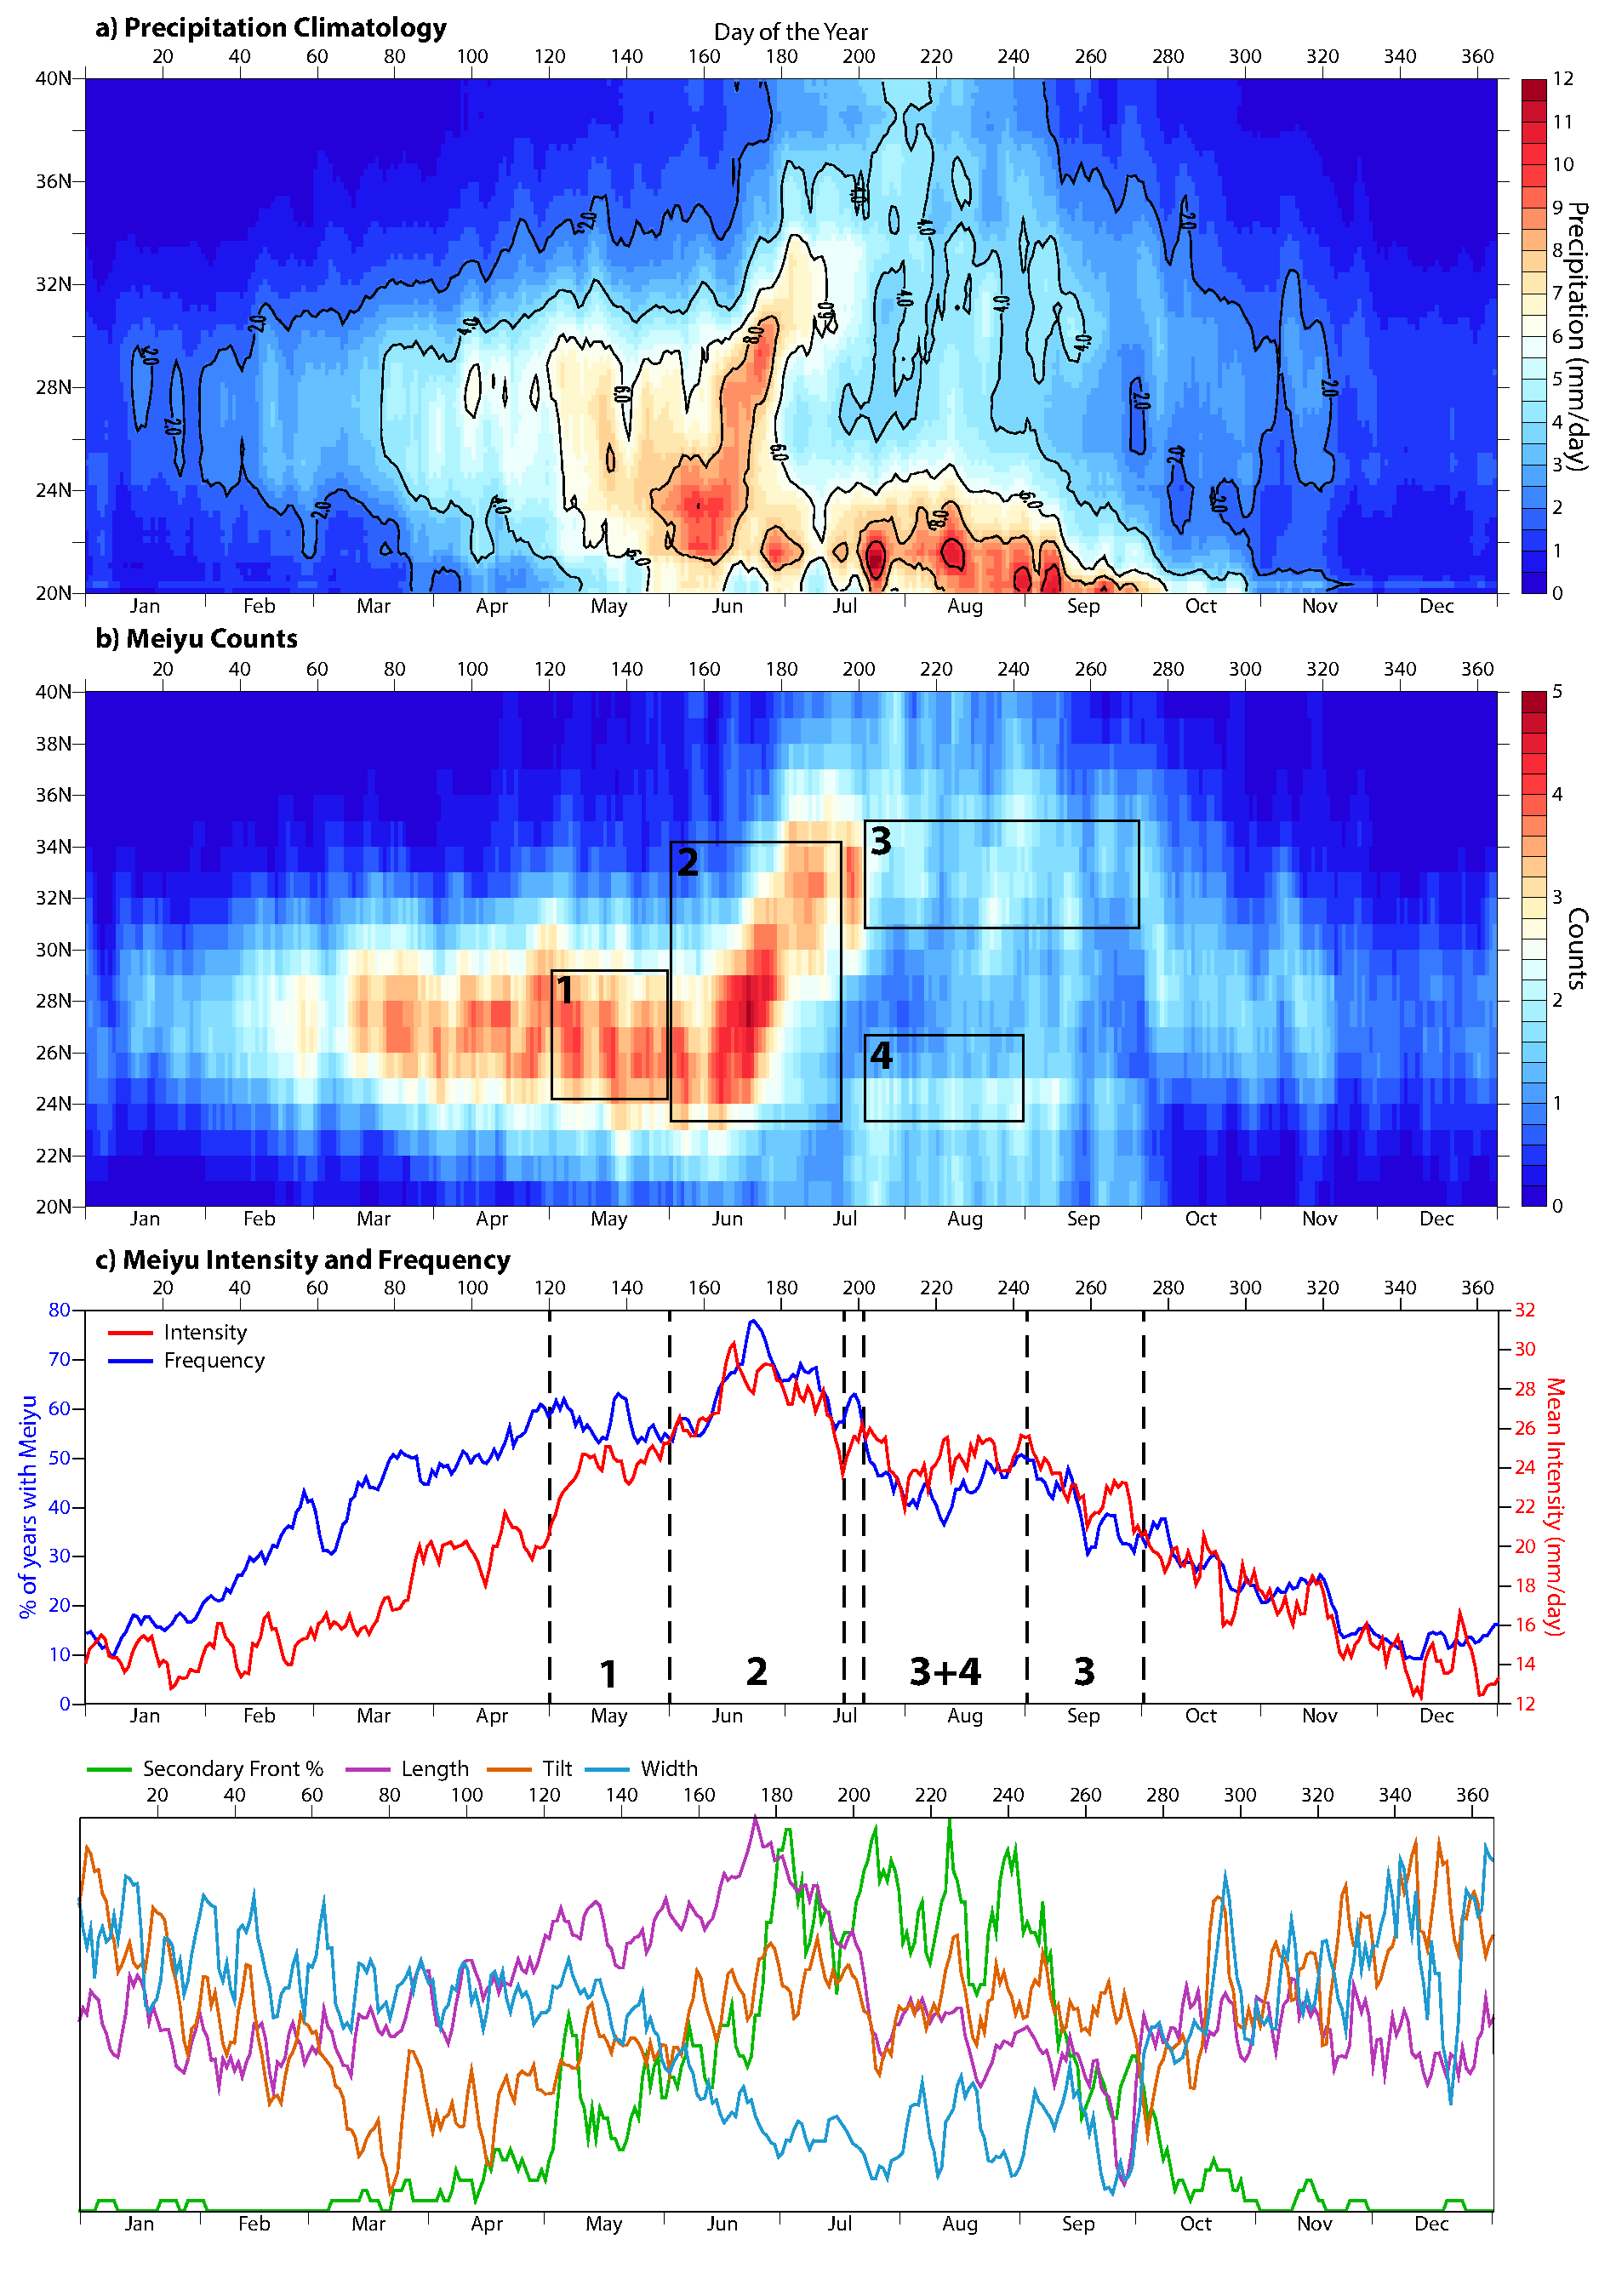
\includegraphics[width=36pc]{fig1_dingchan.pdf}
\caption{Climatology of the Meiyu Front, 1951-2007. 1) Pre-Meiyu 2) Meiyu 3) Cyclone season in Southern China 4) Storms advected by summer jet}
\label{figure_label}
\end{figure}

\end{document}

%%%%%%%%%%%%%%%%%%%%%%%%%%%%%%%%%%%%%%%%%%%%%%%%%%%%%%%%%%%%%%%

More Information and Advice:

%% ------------------------------------------------------------------------ %%
%
%  SECTION HEADS
%
%% ------------------------------------------------------------------------ %%

% Capitalize the first letter of each word (except for
% prepositions, conjunctions, and articles that are
% three or fewer letters).

% AGU follows standard outline style; therefore, there cannot be a section 1 without
% a section 2, or a section 2.3.1 without a section 2.3.2.
% Please make sure your section numbers are balanced.
% ---------------
% Level 1 head
%
% Use the \section{} command to identify level 1 heads;
% type the appropriate head wording between the curly
% brackets, as shown below.
%
%An example:
%\section{Level 1 Head: Introduction}
%
% ---------------
% Level 2 head
%
% Use the \subsection{} command to identify level 2 heads.
%An example:
%\subsection{Level 2 Head}
%
% ---------------
% Level 3 head
%
% Use the \subsubsection{} command to identify level 3 heads
%An example:
%\subsubsection{Level 3 Head}
%
%---------------
% Level 4 head
%
% Use the \subsubsubsection{} command to identify level 3 heads
% An example:
%\subsubsubsection{Level 4 Head} An example.
%
%% ------------------------------------------------------------------------ %%
%
%  IN-TEXT LISTS
%
%% ------------------------------------------------------------------------ %%
%
% Do not use bulleted lists; enumerated lists are okay.
% \begin{enumerate}
% \item
% \item
% \item
% \end{enumerate}
%
%% ------------------------------------------------------------------------ %%
%
%  EQUATIONS
%
%% ------------------------------------------------------------------------ %%

% Single-line equations are centered.
% Equation arrays will appear left-aligned.

Math coded inside display math mode \[ ...\]
 will not be numbered, e.g.,:
 \[ x^2=y^2 + z^2\]

 Math coded inside \begin{equation} and \end{equation} will
 be automatically numbered, e.g.,:
 \begin{equation}
 x^2=y^2 + z^2
 \end{equation}

% IF YOU HAVE MULTI-LINE EQUATIONS, PLEASE
% BREAK THE EQUATIONS INTO TWO OR MORE LINES
% OF SINGLE COLUMN WIDTH (20 pc, 8.3 cm)
% using double backslashes (\\).

% To create multiline equations, use the
% \begin{eqnarray} and \end{eqnarray} environment
% as demonstrated below.
\begin{eqnarray}
  x_{1} & = & (x - x_{0}) \cos \Theta \nonumber \\
        && + (y - y_{0}) \sin \Theta  \nonumber \\
  y_{1} & = & -(x - x_{0}) \sin \Theta \nonumber \\
        && + (y - y_{0}) \cos \Theta.
\end{eqnarray}

%If you don't want an equation number, use the star form:
%\begin{eqnarray*}...\end{eqnarray*}

% Break each line at a sign of operation
% (+, -, etc.) if possible, with the sign of operation
% on the new line.

% Indent second and subsequent lines to align with
% the first character following the equal sign on the
% first line.

% Use an \hspace{} command to insert horizontal space
% into your equation if necessary. Place an appropriate
% unit of measure between the curly braces, e.g.
% \hspace{1in}; you may have to experiment to achieve
% the correct amount of space.


%% ------------------------------------------------------------------------ %%
%
%  EQUATION NUMBERING: COUNTER
%
%% ------------------------------------------------------------------------ %%

% You may change equation numbering by resetting
% the equation counter or by explicitly numbering
% an equation.

% To explicitly number an equation, type \eqnum{}
% (with the desired number between the brackets)
% after the \begin{equation} or \begin{eqnarray}
% command.  The \eqnum{} command will affect only
% the equation it appears with; LaTeX will number
% any equations appearing later in the manuscript
% according to the equation counter.
%

% If you have a multiline equation that needs only
% one equation number, use a \nonumber command in
% front of the double backslashes (\\) as shown in
% the multiline equation above.

%% ------------------------------------------------------------------------ %%
%
%  SIDEWAYS FIGURE AND TABLE EXAMPLES
%
%% ------------------------------------------------------------------------ %%
%
% For tables and figures, add \usepackage{rotating} to the paper and add the rotating.sty file to the folder.
% AGU prefers the use of {sidewaystable} over {landscapetable} as it causes fewer problems.
%
% \begin{sidewaysfigure}
% \includegraphics[width=20pc]{samplefigure.eps}
% \caption{caption here}
% \label{label_here}
% \end{sidewaysfigure}
%
%
%
% \begin{sidewaystable}
% \caption{}
% \begin{tabular}
% Table layout here.
% \end{tabular}
% \end{sidewaystable}
%
%

